\documentclass[a4paper,12pt,frenchb]{article}

\input{../../commons.tex.inc}

\title{Évaluation : théoèrme des valeurs intermédiaires}
\author{semaine \no{49} -- 12\up{ième} semaine de cours}
\date{4 décembre 2017}

\SetWatermarkText{}
\parindent0pt

\begin{document}


\maketitle

\thispagestyle{fancy}

\begin{question}[subtitle={expo}]
  \begin{enumerate}
    \item On considère une fonction $f$ telle que pour tout $x$ réel, $f'(x)
      = f(x)$. Donner $[x \mapsto f(-x)]'$ et $[x \mapsto f(x + b)]'$.
    \item Pour tout $x$ réel, on note $e^x$ la fonction exponentielle.
      \begin{enumerate}
        \item Que vaut $e^0$ ?
        \item Transformer $e^{- 3x + 2}$ et $\dfrac{e^{-2x}}{e^{-3}}$.
        \item Résoudre $e^{-x^2} = e$
        \item Que pensez vous de l'inéquation $e^{-3x} < 0$ ?
      \end{enumerate}
  \end{enumerate}
\end{question}

\begin{question}[subtitle={espace}]

On considère le cube ABCDEFGH représenté ci-dessous.

On définit les points I et J respectivement par $\vv{\text{HI}} = \dfrac{3}{4} \vv{\text{HG}}$ et $\vv{\text{JG}} = \dfrac{1}{4} \vv{\text{CG}}$.

%\begin{center}
%\psset{unit=1cm}
%\begin{pspicture}(8,8.25)
%\psframe(0.5,0.5)(5,5)
%\psline(5,0.5)(7,2.7)(7,7.2)(2.5,7.2)(0.5,5)
%\psline(5,5)(7,7.2)
%\psline[linestyle=dashed](0.5,0.5)(2.5,2.7)(7,2.7)
%\psline[linestyle=dashed](2.5,2.7)(2.5,7.2)
%\uput[ur](2.5,2.7){A} \uput[r](7,2.7){B} \uput[ul](5,0.5){C} 
%\uput[ul](0.5,0.5){D} \uput[ul](2.5,7.2){E} \uput[ur](7,7.2){F} 
%\uput[r](5,5){G} \uput[ul](0.5,5){H} \uput[u](3.875,5){I}
%\psdots(5,0.5)(7,2.7)(7,7.2)(2.5,7.2)(0.5,5)(5,5)(3.875,5)(5,3.875)(2.5,2.7)(0.5,0.5) 
%\uput[r](5,3.875){J} 
%\end{pspicture}
%\end{center}

\begin{enumerate}
\item \textbf{Sur le document réponse donné en annexe, à rendre avec la copie}, tracer, sans justifier, la section du cube par le plan (IJK) où K est un point du segment [BF].
\item \textbf{Sur le document réponse donné en annexe, à rendre avec la copie}, tracer, sans justifier, la section du cube par le plan (IJL) où L est un point de la droite (BF).
\item Existe-t-il un point P de la droite (BF) tel que la section du cube par le plan (IJP)
soit un triangle équilatéral ? Justifier votre réponse.
\end{enumerate}

\pagebreak

\begin{center}
  \vspace{3cm}
  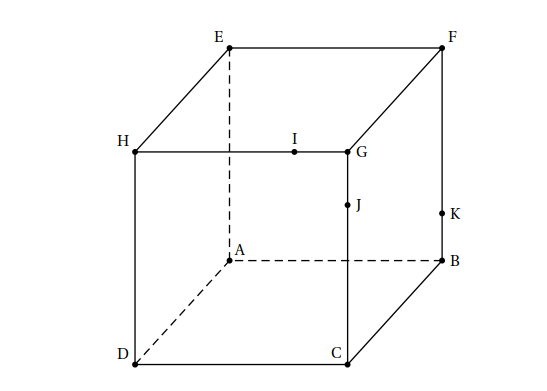
\includegraphics{Screenshot_20171203_185353.png}

  \vspace{4cm}

  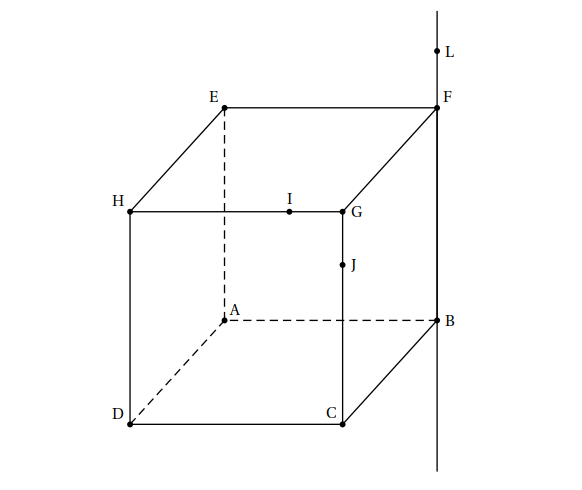
\includegraphics{Screenshot_20171203_185411.png}

  \vspace{3cm}
\end{center}

\end{question}

\end{document}
